\section[Ampere's Law Exercise: An Infinite Current Sheet]{Amp\`ere's Law Exercise: An Infinite Current Sheet}
\begin{comment}
This lab was written by Ted Bunn for spring of 2016.  It was edited slightly by Matt Trawick for this manual in April 2016.

\end{comment}

\makelabheader %(Space for student name, etc., defined in master.tex)

\bigskip

\textbf{Introduction}

Imagine an infinite plane, with charges flowing uniformly across it,
all in the same direction. You're going to find out what sort of
magnetic field is produced by such a ``current sheet.''\footnote{In
case you're wondering, there are actual systems like this in nature.
There aren't any \textit{infinite} current sheets, but in the outer
layers of the Sun, and in many other places, there are \textit{large}
current sheets, for which the results we'll get here provide quite a good
approximation.}

Here's one way to imagine an infinite current sheet. Imagine infinitely
many infinitely long straight wires, all placed right next to each other
in a plane. Each wire carries the same current $I$. This picture shows
a cross section of a bunch of those wires. Each one is carrying current
straight out of the page toward you. You should imagine that each wire
is infinite, and that they extend infinitely far to the left and right.
Let $n$ be the number of wires per unit length.

\bigskip\bigskip

\centerline{
\includegraphics{amperes_law_infinite_sheet/wires_with_dot.eps}}

\bigskip\bigskip

Our goal is to figure out the magnitude and direction of the magnetic field
at the location of the dot above the wires.

\textbf{Activity 1: Finding the Direction}


(a) What is the direction of the magnetic
field at the dot that would be produced by only the one wire that lies directly below
the dot?  Sketch it on the figure above.

(b) Now consider one of the other wires,
say one that is five wires to the left of the dot.
What is the direction of the magnetic field at the point produced by this 
wire? (You don't need to give a precise angle here; just a sketch on the figure is fine.)

(c) Now what about the wire that is five wires to the right of the dot?
What is the direction of the magnetic field at the dot due to this wire?  (Add it to your sketch.)

(d) If you added up the magnetic fields due to the wires in the two
previous questions, in which way would the resultant vector point?
\answerspace{0.5in}

(e) If you added up the magnetic fields due to \textit{all} the wires,
which way would the resultant vector point?
\answerspace{0.5in}

The answer to the last question is the direction of $\vec B$ at 
the location of the dot.

(f) If you moved the dot some distance to the left or right,
would the magnetic field at the dot change? Why not?
\answerspace{0.5in}

(g) If you considered a point \textit{below} the wires instead of
above them, the same distance away as the dot, what would the
direction of the magnetic field be?
\answerspace{0.5in}

(h) On the figure below, draw a series of at least four magnetic field lines showing the direction of the magnetic field everywhere above and below the sheet of wires.
\begin{center}
\centerline{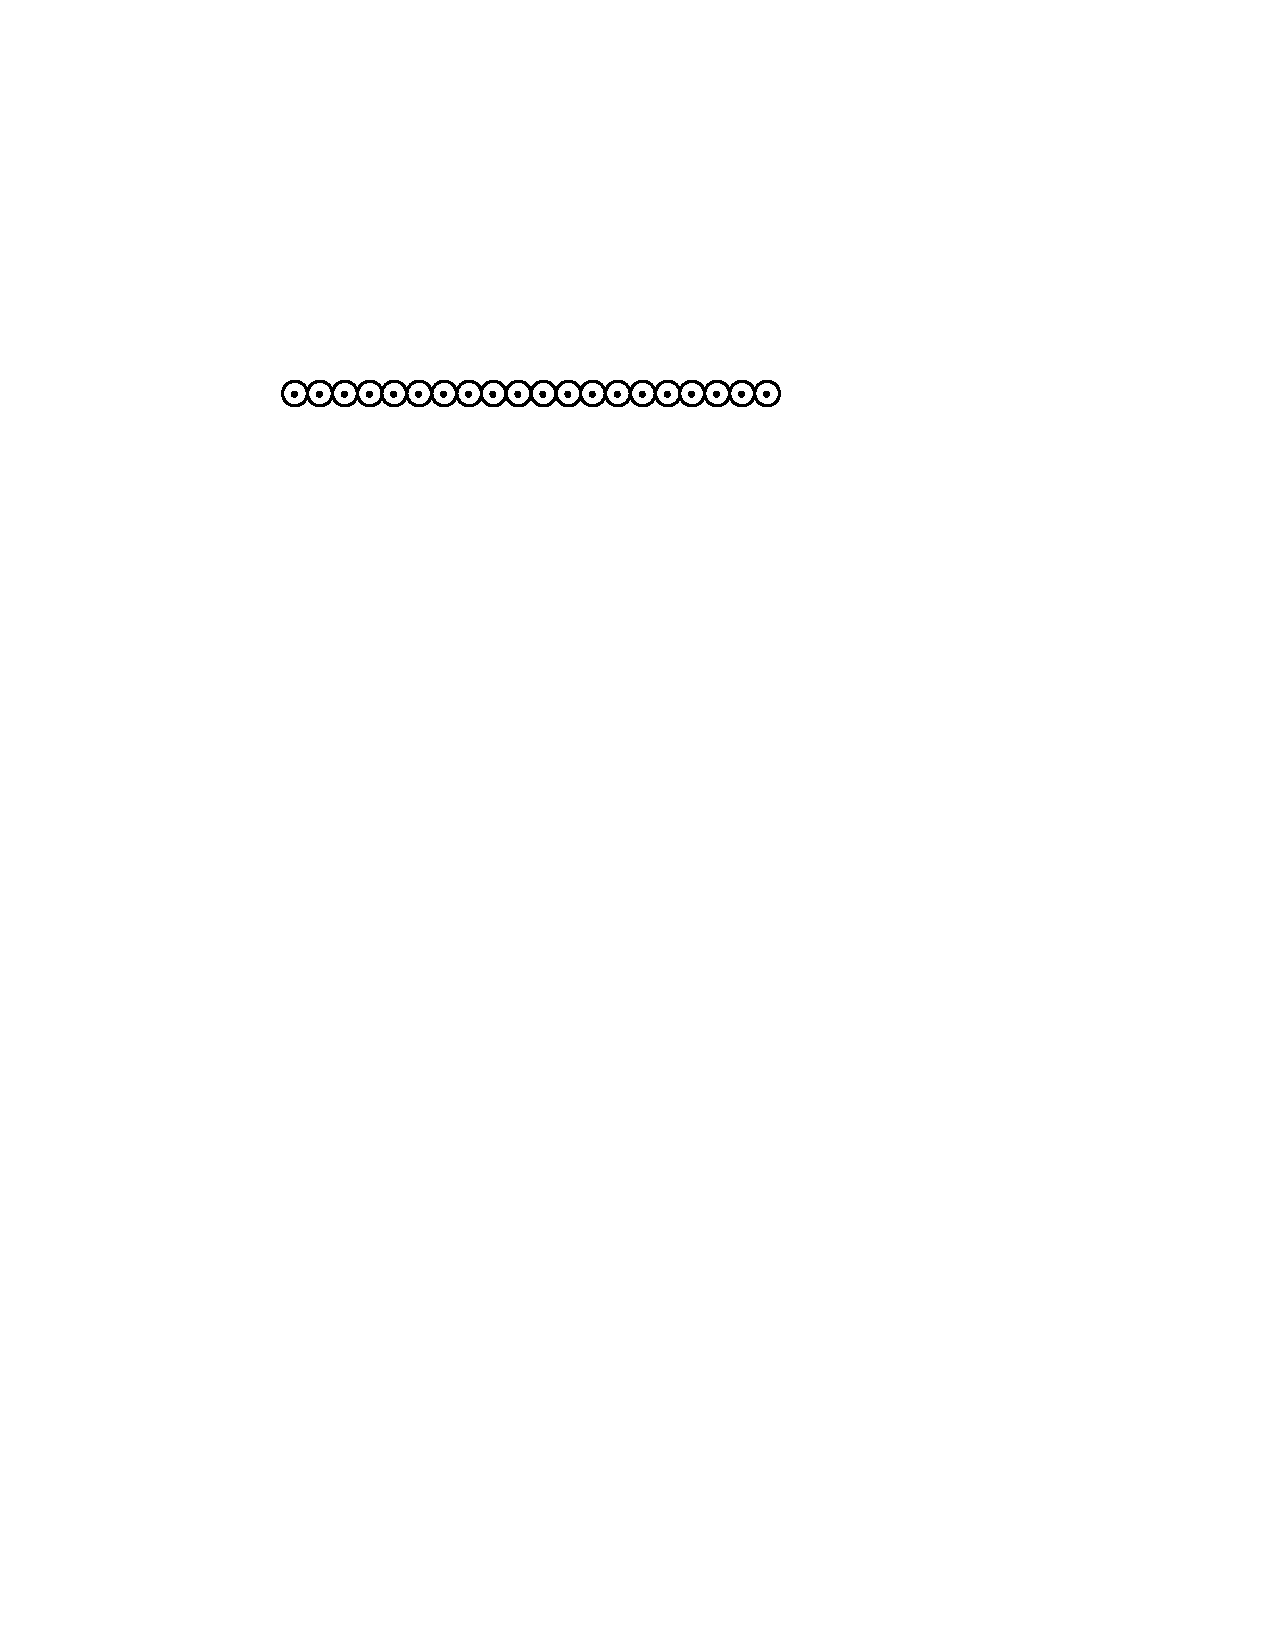
\includegraphics{amperes_law_infinite_sheet/wires_without_dot.pdf}}
\end{center}

\textbf{Activity 2: Using Ampere's Law to Find the Magnitude}

Now let's figure out the magnitude of the field $B$ at the location of the dot.
We're going to apply Amp\`ere's law,
\begin{equation*}
\oint \vv{B}\cdot \vv{ds} = \mu_0 I_{enc}
\end{equation*}
by integrating around \textit{one} of the closed paths in the digram below.

\begin{center}

\includegraphics{amperes_law_infinite_sheet/wires_with_dot_and_paths.eps}
\end{center}

Amp\`ere's law is \textit{true} for ALL of the paths in the picture.  But it's only \textit{useful} to us here if it will help us to calculate $B$.  In general, we want to pick a path that has these properties:
\begin{itemize}[nosep]
\item The path should go through the point where we want to know the field.
\item The path should enclose some current.
\item The vectors $\vv{B}$ and $\vv{ds}$ should always be either \textit{parallel} or \textit{perpendicular} to each other, so that $\vv{B}\cdot \vv{ds}$ is easy to calculate.  (Remember, $\vv{ds}$ points along the dotted line path we're integrating around.)
\end{itemize}
%\newpage

(a) The figure above shows three paths: a circle, a rectangle, and \ldots a third one.  Bearing in mind the magnetic field lines you drew at then end of Activity 1, which path satisifies all three criteria listed above?
\answerspace{0.3in}

\pagebreak[3]
(b) Let's work on the right side of the Amp\`ere's law equation first.  We already said the number of wires per unit length is $n$, and each wire carries current $I$.  If we suppose the rectangular path has a width of $\ell$, how many wires are \textit{enclosed} inside the path?  (Don't just count the wires in the lousy picture; we're looking for 
an algebraic expression in terms of stuff like $n$ and $\ell$.)
\answerspace{0.3in}

(c) How much current $I_{enc}$ is \textit{enclosed} by the path?
\answerspace{0.5in}

(d) Now we'll work on the left side of Amp\`ere's law, $\oint \vv {B}\cdot \vv{ds}$.  Evaluate the integral, 
expressing the result in terms of some
or all of the quantities $B$ (which is what we're trying
to find), $\ell$, and maybe the height $r$ of the dot above the wire.  In order to do this, you'll have to consider
the integral along each of the four sides of the rectangle,
and add them up.
\answerspace{1.3in}

(e) In the last two questions, you worked out expressions
for the two sides of Amp\`ere's Law. Set them equal to each other
and solve for $B$.
\answerspace{1in}

\centerline{\textit{We're done! That's the expression for the magnetic field produced 
by a current sheet.}  :-)}

(f) We made up our path to have an arbitrary width $\ell$.  In the end, did the magnetic field $B$ depend on $\ell$, bearing in mind that you'd be screwed if the field you found depended on some length you imagined in your head?
\answerspace{0.4in}

(g) Does the strength of the magnetic field $B$ depend on the
distance $r$ from the sheet?  Can you think of another case you've seen where a field $\vv{E}$ or $\vv{B}$ depends (or doesn't depend) on a distance $r$ in the same way?
\answerspace{0.4in}
